
\documentclass{proposal}
\usepackage{verbatim}
\usepackage{graphicx}
\graphicspath{ {./plot/} }
\usepackage{svg}

\degree{Doctor of Philosophy}
\department{Electrical Engineering}
\gradyear{2019}
\author{Jiexin Gao}
\title{Predicting in vivo RNA Secondary Structure}

\setcounter{tocdepth}{2}

\flushbottom

\begin{document}

\begin{preliminary}

\maketitle

\begin{abstract}



\end{abstract}

\tableofcontents

\end{preliminary}





\chapter{Introduction}
%\addcontentsline{toc}{chapter}{Introduction}




Although once believed to be an intermediate molecule that serves as messenger between DNA and protein,
RNA is now known to be involved in many aspects in gene regulation and expression.
Unlike DNA which forms stable double helix, RNA predominantly stays single-stranded and folds onto itself by
forming base pairs via hydrogen bonds, including Watson-Crick pair A-U, G-C and non-canonical TODO pair A-U.
Nearby paired and unpaired bases  \iffalse forms stems and loops, \fi and further leads to the formation TODO of
hairpins, bulges, internal loops, Multi loops and pseudoknots.
In addition, secondary structures within an RNA molecule can interact via non-covalent bond, to form tertiary structure.


RNA secondary and tertiary structure play key roles in regulating both coding and nocoding transcripts,
and affect all steps of gene regulation including transcription, splicing, polyadenylation, translation,
localization and stability\cite{wan2011understanding}.
Over the past few years, combination of RNA structure probing and high throughput sequencing has enabled
the discovery? of genome-wide RNA structural in multiple organisms and cell types,
??? better understanding of the relationship between RNA structure and function.


\section{RNA secondary structure and gene regulation}


\subsection*{Polyadenylation}

Ding et. al\cite{ding2014vivo} used Structure-Seq (TODO review) to study the genome-wide RNA structure of
\textit{Arabidopsis thaliana} seedlings \textit{in vivo} and discovered a pattern around alternative polyadenylation sites across $5959$ mRNAs.
As shown in Fig \ref{fig:poly_a}, region upstream of the site (-15nt to -2nt) is significantly more structured, as indicated by lower reactivity,
and region downstream of the site (-1nt to +5nt) is significantly less structured, as indicated by higher reactivity.
This

\begin{figure}[h!]
    \centering
    \includegraphics[width=0.6\textwidth]{poly_a.png}
    \caption{RNA structure around alternative polyadenylation sites in \textit{Arabidopsis thaliana}. From Ding et. al\cite{ding2014vivo}.}
    \label{fig:poly_a}
    \centering
\end{figure}


\subsection*{Transcription}

Kertesz et. al\cite{kertesz2010genome} performed in vitro profiling of the budding yeast
(\textit{Saccharomyces cerevisiae}) RNA structure using PARS (TODO).
Averaging PARS scores across more than $3000$ mRNAs revealed a unique pattern across the transcript (Fig \ref{fig:yeast_cds_utr}):
 the UTRs are less structured than the CDS, both start and stop codon are significantly more accessible,
and the coding region exhibits a three nucleotide periodical pattern,
where the first nucleotide is more accessible and the second one is less accessible.

In contrary, although RNAs in human show a similar start/stop codon accessibility and CDS periodicity,
it was observed that UTRs are only slightly less structured than CDS\cite{wan2014landscape}.  (TODO, other paper says more structured?)


\begin{figure}[h!]
    \centering
    \includegraphics[width=0.8\textwidth]{yeast_cds_utr.png}
    \caption{Yeast RNA structure differ in CDS and UTR. From Kertesz et. al\cite{kertesz2010genome}.}
    \label{fig:yeast_cds_utr}
    \centering
\end{figure}


\subsection*{Splicing}

Wan et. al\cite{wan2014landscape} analyzed human lymphoblastoid cell lines from a parent-offspring trio by PARS (TODO review),
and observed less structure at AG dinucleotide in the upstream exon donor site,
and more structure at the first nucleotide in the downstream acceptor site, as shown in Fig \ref{fig:exon_exon_junction}.
Potential role in efficient splicesome assembly.


\begin{figure}[h!]
    \centering
    \includegraphics[width=0.4\textwidth]{exon_exon_junction.png}
    \caption{RNA structure at exon-exon junction in human lymphoblastoid cell lines. From Wan et. al\cite{wan2014landscape}.}
    \label{fig:exon_exon_junction}
    \centering
\end{figure}


\subsection*{Translation}

Kertesz et. al\cite{kertesz2010genome} reported a small but significant anti-correlation between PARS scores 10bp upstream
of the start codon and ribosome density throughout the transcript.
In addition, genes where 5'UTRs are less structured than the beginning of the coding region also show a tendency towards higher ribosome density.

\subsection*{Localization}

Kertesz et. al\cite{kertesz2010genome} discovered increased structure in coding region for genes
whose encoded proteins localize to distinct cellular domains or function in specific metabolic pathways.
On the other hand, ribosomal transcripts show less structure in UTR and CDS (Fig \ref{fig:yeast_localization}).



\begin{figure}[h!]
    \centering
    \includegraphics[width=0.4\textwidth]{yeast_localization.png}
    \caption{RNA structure in CDS and UTR affects localization in yeast. From Kertesz et. al\cite{kertesz2010genome}.}
    \label{fig:yeast_localization}
    \centering
\end{figure}



\subsection*{Stability}


Kertesz et. al\cite{kertesz2010genome} discribed how RNA structure in UTR regulates gene expression during heat shock in order to conserve energy.
Certain class of genes (e.g. ribosomal encoding RPL1A) with less UTR structure becomes unfolded with increased temperature,
which allows degradation by exosome, thus tuning down translation.
On the other hand, genes with more UTR structure like chaperones and unfolded response proteins (e.g. HAC1 and PTC2) remain stable and expressed (Fig \ref{fig:yeast_stability}).

\begin{figure}[h!]
    \centering
    \includegraphics[width=0.6\textwidth]{yeast_stability.png}
    \caption{Yeast gene expression regulation via RNA structure during heat shock. From Mortimer et. al\cite{mortimer2014insights}.}
    \label{fig:yeast_stability}
    \centering
\end{figure}


\section{High throughput probing of RNS secondary structure}


It has been demonstrated in various organisms that in vivo structure can differ significantly from in vitro.
In a living cell environment, the presence of proteins,  ?ligand, salt, temperature?, all affects RNA structure,
and he precise reconstruction of these conditions in vitro is almost impossible.
Rouskin et al.\cite{rouskin2014genome} studied yeast RNA structure and found that RNAs are less structured in vivo than in vitro.
Moreover, they observed that structures unfold when $Mg^{2+}$ is lowered in vitro,
and more structured regions emerge when cell is depleted of ATP in vivo.
(which underscores the importance of in vivo probing that captures the specific physiological condition of the cell type of interest)


vast number of non coding RNAs (still being discovered)

constran prediction using data

whereas

disease

%relationship to gene regulation, splicing, polyA, half life, stability, translation (uORF)
%cite papers
%
%ribosnitch
%
%RNA structure & disease
%
%RNA structure & interaction with protein
%
%secondary v.s. tertiary structure
%
%what determines RNA structure, focus on vivo
%
%review thermodynamic based models
%
%context-free-grammar based models
%
%conservation based models
%
%review DMfold-like models
%
%why do we need a computational model for in vivo folding?
%
%- prediction long RNA structure without the need to probe them (any limitation in probing long RNAs?)
%
%- predict structure of RNA with low abundance (hard to measure, need to do targetted sequencing)
%
%- predict structure of novel RNA, e.g. with mutation,
%
%- structure representation for transfer learning





%review different experimental technique, comparison, pros v.s. cons
%
%vivo v.s. vitro
%
%enzymes v.s. chemicals
%
%
%K562 and yeast DMS data\cite{rouskin2014genome}
%
%Mouse embryonic stem cell v6.5 icSHAPE data\cite{spitale2015structural}
%
%Yeast ModSeq validation data\cite{talkish2014mod}
%
%Hek293 and mouse validation data (different compartments)\cite{sun2019rna}



\section{Deep neural network}

%sequence to sequence models, RNN, LSTM, transformer
%
%residual net, dense net
%
%cite spliceAI

\chapter{Yeast Model}

\section{Training Dataset}

To model in vivo RNA secondary structure, we compiled training data from \cite{rouskin2014genome}.
In this study, yeast strain was treated with dimethyl sulphate (DMS), which reacts with unpaired adenine and cytosine bases.
The pool of modified RNAs were fragmented and sequenced.
Since DMS modification blocks reverse transcription, 
number of reads (TODO stops?) at each position is indicative of relative accessibility of that site.

Raw count data was downloaded from GSE45803 (\verb|GSE45803_Feb13_VivoAllextra_1_15_PLUS.wig.gz| and \verb|GSE45803_Feb13_VivoAllextra_1_15_Minus.wig.gz|).
The authors aligned 25nt of each read to a non-redundant set of RefSeq transcripts,
where each gene is represented by its longest protein-coding transcript.
Only uniquely mapped reads with less than 2 mismatches were retained,
and the authors further filtered out aligned reads whose RT stop is not A/C.
The count at each position represents the combined number of RT stops at that site, across $4$ biological replicates.

To construct training dataset, Saccharomyces cerevisiae assembly R61 (secCer2) RefSeq gene annotation was used to extract mRNA sequences.
For each transcript, we first extract the raw read count for all adenine (A) and cytosine (C) bases
(A/C positions with no RT stop coverage were set to a count of $0$),
and applied $90\%$ Winsorization to remove outliers.
Specifically, for each non-overlapping window of 100 A/C bases, values above the $95\%$ percentile was set to the $95\%$ percentile,
and values below the $5\%$ percentile was set to the $5\%$ percentile.
Then, all values within this window were divided by the max, to obtain values between $0$ and $1$.

%To avoid inclusion of low quality data points in the training set, we filtered out transcripts whose A/C coverage is below $0.2$,
%where A/C coverage is defined as

%We used the poly-A selected yeast data to compile training dataset consists of mRNAs.

%Alignments were performed with bowtie using the first 25 nt of each read
%Reads were first aligned to the ribosomal RNA and the unaligned reads were then aligned to the genome
%reads were filtered for unique map to the genome and no mismatches
%reads were filtered for reverse transcriptase stops at As and Cs only
%Genome_build: Saccharomyces cerevisiae assembly R61 (UCSC: sacCer2).
%Supplementary_files_format_and_content: The position number directly indicates the DMS modified position starting at 1. Raw reads for each replicates were combined together in wiggle format. Separate files are provided for positive and negative strand maching reads.


\section{Deep neural network}


We construct a deep neural network to predict reactivity at single base resolution from RNA sequence context.
We use an architecture similar to DenseNet\cite{huang2017densely},
in which we've removed the pooling layers, to maintain the spatial resolution throughout the depth of the neural network.

%\begin{figure}[htbp]
%  \centering
%  \includesvg{plot/proposal_dense_net.svg}
%  \caption{svg image}
%\end{figure}

\begin{figure}
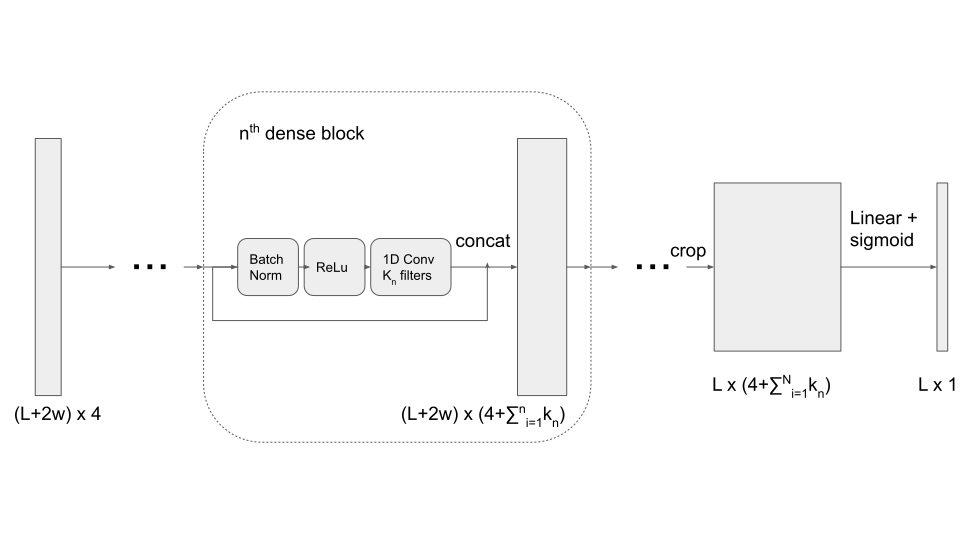
\includegraphics[width=\textwidth]{proposal_dense_net.png}
\caption{Densely connected neural network used for the yeast model}
\label{fig:dense_net}
\centering
\end{figure}

As shown in Fig\ref{fig:dense_net}, to make inference on a stretch of RNA sequence of length $L$,
we need to pad the sequence with $w$ bases on each side. (TODO explanation + how to calculate $w$)
Input consists of the one-hot encoded, padded sequence,
where $A, C, G, U$ bases are encoded as $[1, 0, 0, 0], [0, 1, 0, 0], [0, 0, 1, 0], [0, 0, 0, 1]$, respectively.
The encoded input is then passed through multiple dense blocks,
where each block consists of four components:

\begin{enumerate}
    \item Batch Normalization
    \item ReLu nonlinear activation
    \item 1D Convolution
    \item Concatenation of the block input to the output of convolution
\end{enumerate}

%- {dilation: 1, filter_width: 16, num_filter: 128}
%- {dilation: 2, filter_width: 16, num_filter: 128}
%- {dilation: 4, filter_width: 16, num_filter: 256}
%- {dilation: 8, filter_width: 16, num_filter: 256}
%- {dilation: 16, filter_width: 16, num_filter: 512}

\begin{table}[h!]
    \centering
    \begin{tabular}{||c c c c||}
        \hline
        Block number & Number of filters & Filter width & Dilation rate \\ [0.5ex]
        \hline\hline
        1 & 128 & 16 & 1 \\
        \hline
        2 & 128 & 16 & 2 \\
        \hline
        3 & 256 & 16 & 4 \\
        \hline
        4 & 256 & 16 & 8 \\
        \hline
        5 & 512 & 16 & 16 \\ [1ex]
        \hline
    \end{tabular}
    \caption{Dense block parameters}
    \label{table:conv_layer_params}
\end{table}

We use $5$ dense blocks in this work. The parameter of each layer is as shown in Table\ref{table:conv_layer_params}.
Densely connected block has the advantage that each block receives input from all preceding blocks,
and passes its output to all successive blocks.
The output of the last dense block essentially represents the features learnt from input at multiple resolutions.

The final dense block output is then cropped to account for the input padding,
and then passed through a fully connected layer with sigmoid activation, along the feature dimension.


\section{Training}

%- [chrM, chrVIII, chrII, chrXV]
%- [chrI, chrV, chrXIII, chrIV]
%- [chrVI, chrXI, chrXVI]
%- [chrIII, chrX, chrXII]
%- [chrIX, chrXIV, chrVII]

\begin{table}[h!]
    \centering
    \begin{tabular}{||c c||}
        \hline
        Fold number & Chromosomes \\ [0.5ex]
        \hline\hline
        1 & chrM, chrVIII, chrII, chrXV \\
        \hline
        2 & chrI, chrV, chrXIII, chrIV \\
        \hline
        3 & chrVI, chrXI, chrXVI \\
        \hline
        4 & chrIII, chrX, chrXII \\
        \hline
        5 & chrIX, chrXIV, chrVII \\ [1ex]
        \hline
    \end{tabular}
    \caption{Chromosomes used for each fold}
    \label{table:fold_chrom_split}
\end{table}


We use 5-fold cross validation, where the folds are splited by chromosomes, as shown in Table \ref{table:fold_chrom_split}.

Normalized data points (between $0$ and $1$) are used as soft targets without being converted to binary labels,
and models were trained using a masked cross-entropy loss, as described below.

Due to the nature of DMS modification, G/T bases has no coverage,
thus should be excluded from the calculation of the loss and the gradient.
This is achieve by first computing the per position cross-entropy loss between the prediction and the target,
then multiply it with a binary mask with the same shape as the target array.
Positions with G/T bases are being set to $0$ in the mask, while positions with A/C bases are $1$.
The masked loss are then summed over positions, and minibatch dimension, to calculate the loss for the current minibatch and the gradient for back propagation.

Models were trained using fixed sequence length of $50$ (before padding, sequence length at inference time can be variable),
minibatch size of $10$, Adam optimizer with learning rate $0.0001$ and momentum $0.9$.
To prevent the models from overfitting, L1 and L2 regularizers with weight $0.000001$ was added to the loss,
and training is stopped if validation loss hasn't improved over the last $10$ epochs.

We trained $5$ models, each using one of the folds as validation data, and the rest as training data.


\section{Performance}


\subsection{Cross-validation performance on training dataset}

We first evaluate the model performance on training dataset.
For each transcript, we used the model that wasn't trained on its chromosome to make prediction for all A/C bases.
We computed the Spearman correlation between the prediction and the target for each transcript.
Fig \ref{fig:yeast_cv_performance} shows the distribution of Spearman correlation across all transcripts.

\begin{figure}[h!]
\includegraphics[width=\textwidth]{yeast_cv_performance.png}
\caption{Densely connected neural network used for the yeast model}
\label{fig:yeast_cv_performance}
\centering
\end{figure}

\subsection{Ribosomal RNA}

Next we used our model to predict the reactivity for all A/C bases in yeast $18S$ and $15S$ ribosomal RNAs,
both were never seen by the model (neither in the training nor validation set).

Raw read count data for $18S$ and $15S$ was downloaded from GSE45803, and was processed similarly to the training dataset,
since the experimental protocol was identical.

Correlation between prediction and the normalized read count is shown in Fig\ref{fig:yeast_r18_performance} and Fig\ref{fig:yeast_r25_performance},
where each data point is one A/C base in the corresponding transcript.
In comparison, RNAfold (window size $50$ and span $50$) achieves a correlation of $0.3217$ and $0.4529$ for $18S$ and $15S$, respectively.

\begin{figure}[h!]
\includegraphics[width=\textwidth]{yeast_r18_performance.png}
\caption{Densely connected neural network used for the yeast model}
\label{fig:yeast_r18_performance}
\centering
\end{figure}

\begin{figure}[h!]
\includegraphics[width=\textwidth]{yeast_r25_performance.png}
\caption{Densely connected neural network used for the yeast model}
\label{fig:yeast_r25_performance}
\centering
\end{figure}


\subsection{Noncoding RNAs}

To evaluate whether the model generalizes to noncoding transcripts and different experimental protocol,
we processed yeast data from the ModSeq paper\cite{talkish2014mod},
where yeast was treated with DMS or no-DMS (as control),
and the authors identified positions that are significantly modified between treated and control,
in selected noncoding and rRNA transcripts.

For each transcript, we use our models to predict on all A/C positions,
and computed the au-ROC on how well the prediction distinguish the significantly modified bases from the rest.
We also compare the performance of our model to that of RNAfold, as shown in Fig\ref{fig:yeast_modseq_performance}.

\begin{figure}[h!]
\includegraphics[width=\textwidth]{yeast_modseq_performance.png}
\caption{Densely connected neural network used for the yeast model}
\label{fig:yeast_modseq_performance}
\centering
\end{figure}


\section{Future Work}

\begin{itemize}
  \item Improve training and generalization performance, by making use of the raw sequencing data, and biological replicates.
  In additional to counts of RT stops, read coverage at each position can be used to infer the confidence of calling that position paired/unpaired.
  Transcript can be reweighted during training, according to the agreement between different biological reps.

  \item Multi-resolution learning.
\end{itemize}


\chapter{Mouse Model}


\chapter{Human Model}

\chapter{Conclusion and future work}

one dataset that has multiple mods per sequence, so we can reconstruct colleciton of structures

joint learning of accessibility and other data, e.g. chip-seq peaks


\addcontentsline{toc}{chapter}{Bibliography}
\bibliographystyle{plain}
\bibliography{proposal}

\end{document}
